%!TEX program=xelatex
\documentclass[UTF8]{ctexart}

%%%%%% 导入包 %%%%%%
\usepackage{graphicx}
\usepackage{xcolor}
\usepackage{algorithm,algorithmicx}
\usepackage{algpseudocode}
\usepackage{amsmath,amssymb,amsthm}

%%%%%% 算法部分改为中文显示 %%%%%%%%%
\floatname{algorithm}{算法}
\renewcommand{\algorithmicrequire}{\textbf{输入:}}
\renewcommand{\algorithmicensure}{\textbf{输出:}}

%%%% 正文开始 %%%%
\begin{document}

\title{期末作业}
%
\author{陈文宇}

\date{\today}

\maketitle{}


\section{积分近似}
问题重述:
利用复化Gauss公式计算$f(x)=e^{x^{2}+x}$在$[-1,1]$积分的近似值。\\
具体代码,详见附件TheFirstQuestion.c。结果如下:
\begin{figure}[h!]
	\centering
	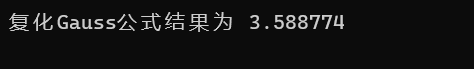
\includegraphics[scale=0.6]{Pic1.png}
\end{figure}

\section{拟合函数}
问题重述:
对于指定基函数,确定$f(x)=e^{x^{2}+x}$在指定拟合点和拟合点函数值且使误差最小的拟合函数,并给出最小误差。

基函数$1,x,x^{2},sin(2x),cos(2x)$是线性无关的,且基函数个数小于拟合点个数,满足哈尔条件,故可以使用线性最小二乘法求解拟合函数。

具体代码,详见附件TheSecondQuestion.c。结果如下:

\begin{figure}[h!]
	\centering
	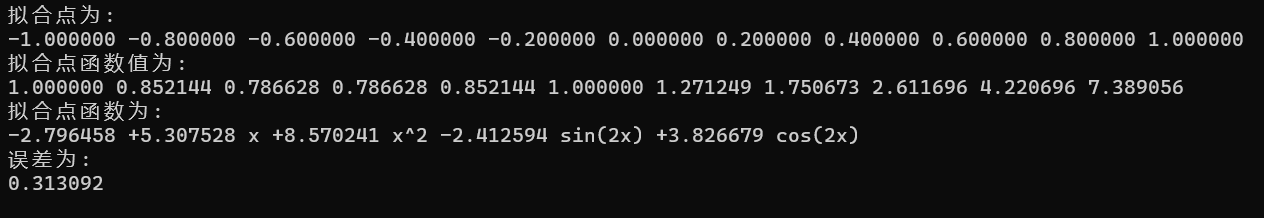
\includegraphics[scale=0.4]{Pic2.png}
\end{figure}

\section{最佳平方逼近函数}
问题重述:
对于指定基函数和积分法,确定$f(x)=e^{x^{2}+x}$的最佳平方逼近函数。

基函数$1,x,x^{2},sin(2x),cos(2x)$是线性无关的,则Gram矩阵是可逆的。利用Gauss积分法可以求解Gram矩阵及右端列向量各个元素的近似值,然后求解线性方程组即可。

具体代码,详见附件TheThirdQuestion.c。结果如下:
\begin{figure}[h!]
	\centering
	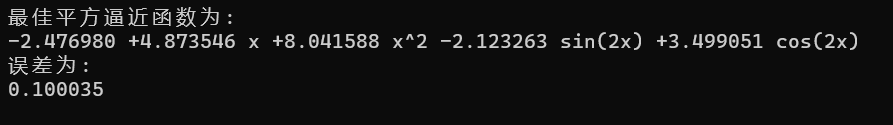
\includegraphics[scale=0.55]{Pic3.png}
\end{figure}

\section{关于第三题的摄动分析}
矩阵A的精确值为
\[
\left(
\begin{matrix}
	2 & 0 & \dfrac{2}{3} & 0 &-sin2 \\
	0 & \dfrac{2}{3} & 0 & -cos2+\dfrac{1}{2}sin2 & 0\\
	\dfrac{2}{3} & 0 & \dfrac{2}{5} & 0 & cos2+\dfrac{1}{2}sin2 \\
	0  & -cos2+\dfrac{1}{2}sin2 & 0 & 1-\dfrac{1}{4}sin4 & 0 \\
	-sin2 & 0 & cos2+\dfrac{1}{2}sin2 & 0 & 1+\dfrac{1}{4}sin4 
\end{matrix}
\right)
\]

由摄动分析理论知,方程组的解对于误差的敏感程度取决于系数矩阵的条件数。由matlab简单函数$cond()$可以计算出系数矩阵的条件数为$140.48$,这不是一个很大的数。

另外,Gauss积分公式在每一小区间上的积分余项为\\
$$R_{n}(f)=\dfrac{f^{(4)}(\xi)}{24}\int_{a}^{b}w^{2}(x)dx$$
利用均值不等式逐段的对$w^{2}(x)$放缩,可以得到$$w^{2}(x)\leqslant (\dfrac{h}{2})^{4}$$
从而可以估计整体的余项:
$$R(f)\leqslant \dfrac{\max \limits_{x\in[-1,1]}|f^{(4)}(x)|}{24} h^{5}$$
当$f^{(4)}(x)$较小时,整体的精度很高。显然,任意两个基函数的乘积函数的四阶导数值都较小。所以Gram矩阵每一元素的精度很高。从而对系数矩阵的扰动很微小,方程的解在这样的扰动下很稳定。所以第三问的结果是可以认可的。

\begin{thebibliography}{99}
	
	\bibitem{Huang2008}{黄明游,冯果忱主编. 数值分析.下册 北京: 高等教育出版社, 2008.1.}
	
\end{thebibliography}

\end{document}
